This test problem simulates an incident flux at a shallow angle to
the bottom edge of a 2-D void region.
This test reveals the diffusivity of a transport scheme in the transverse
direction; artificial diffusion will cause the ``sides'' of a radiation beam,
not just the front, to diffuse.
Table \ref{tab:glance_in_void} summarizes the problem parameters.

%-------------------------------------------------------------------------------
\begin{table}[htb]\caption{Glance-in-Void Test Problem Summary}
\label{tab:glance_in_void}
\centering
\begin{tabular}{l l}\toprule
\emph{Parameter} & \emph{Value}\\\midrule
Domain & $\mathcal{D} = (0,10)^2$\\
Initial Conditions & $u_0(\x)=0$\\
Boundary Conditions & $u(\x,t)=\left\{\begin{array}{c c}
  \frac{\pi}{3} & y = 0, \, t > 0\\
  0             & x = 0, \, t > 0
  \end{array}\right. \eqc$\\
Direction & $\di = (0.868890300722,0.350021174582)$,\\
          & normalized such that $\|\di\| = 1$\\
Cross Section & $\sigma(\x)=0$\\
Source & $q(\x,t)=0$\\
Speed & $\speed=1$\\
\bottomrule\end{tabular}
\end{table}
%-------------------------------------------------------------------------------

This test problem was run on a 64-cell$\times$64-cell mesh.

%with the time step
%size set equal to 


%Table \ref{tab:void_to_absorber_run_parameters} shows the run parameters used
%to obtain the results in this section, Figures \ref{fig:void_to_absorber_2D_fe}
%and \ref{fig:void_to_absorber_2D_ssprk33} show 2-D results for explicit Euler
%and SSPRK33 time discretizations, respectively, and Figure
%\ref{fig:void_to_absorber_3D} shows 3-D results.
%
%From Figure \ref{fig:void_to_absorber_2D_ssprk33}, one can see that the
%Galerkin scheme (which has no artificial dissipation) generates significant
%spurious oscillations perpindicular to the transport direction, even below the
%absorber region. The oscillations are particularly severe along the lower edge
%of the absorber region, where particles/photons are travelling parallel to the
%absorber; this edge has a sharper gradient in the solution than the left edge
%of the absorber region due to the lack of attenuation in this direction, which
%is present for the left edge. Figure \ref{fig:void_to_absorber_2D_ssprk33},
%which uses explicit Euler instead of SSPRK33 does not show the Galerkin plot
%because the oscillations grew without bound, leading to infinite solution
%values. The entropy viscosity scheme is also vulnerable to spurious
%oscillations, although to a lesser extent than the Galerkin scheme.
%
%%-------------------------------------------------------------------------------
%\begin{table}[ht]\caption{Normal Void-to-Absorber Test Problem Run Parameters}
%\label{tab:void_to_absorber_run_parameters}
%\centering
%\begin{tabular}{l l}\toprule
%\emph{Parameter} & \emph{Value}\\\midrule
%Number of Cells & $N_{cell} = 16384$\\
%End Time & $t = 1$\\
%CFL Number & $\nu = 0.5$\\\midrule
%Entropy Function & $\entropy(\scalarsolution) = \frac{1}{2}\scalarsolution^2$\\
%Entropy Residual Coefficient & $\entropyresidualcoef = 0.1$\\
%Entropy Jump Coefficient & $\entropyjumpcoef = 0.1$\\
%\bottomrule\end{tabular}
%\end{table}
%-------------------------------------------------------------------------------
\begin{figure}[ht]
   \centering
   \begin{subfigure}{0.45\textwidth}
      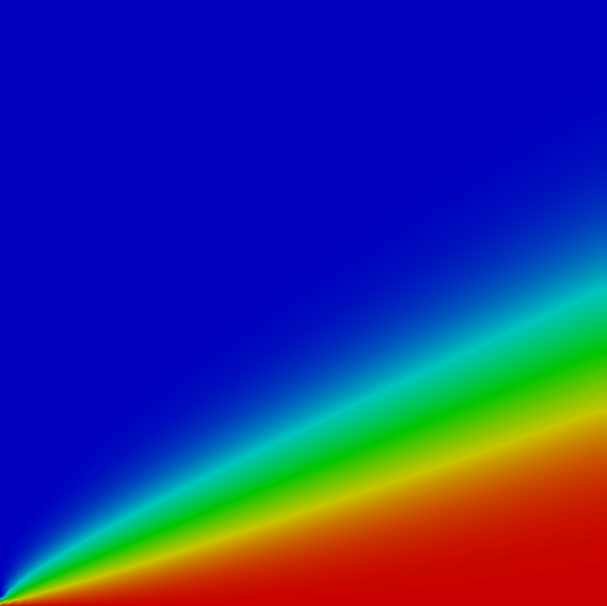
\includegraphics[width=\textwidth]
        {\contentdir/results/transport/glance_in_void/images/DMP_FE.png}
      \caption{Low-Order}
   \end{subfigure}
   \begin{subfigure}{0.45\textwidth}
      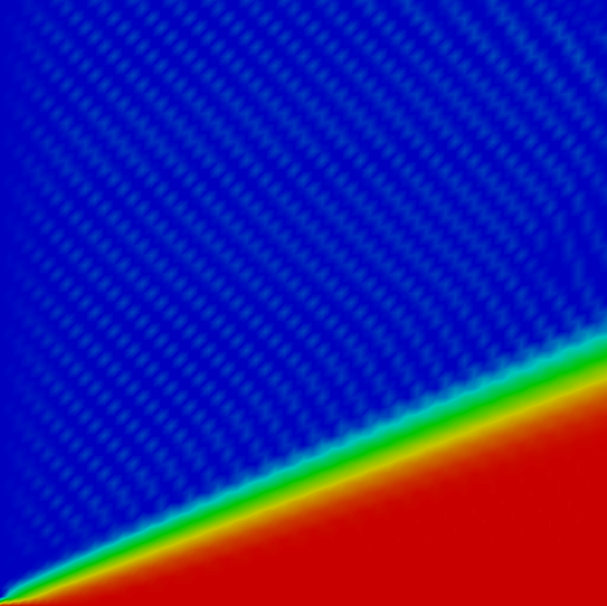
\includegraphics[width=\textwidth]
        {\contentdir/results/transport/glance_in_void/images/EV_FE_cE1.png}
      \caption{EV, $\entropyresidualcoef=1.0$}
   \end{subfigure}
   \begin{subfigure}{0.45\textwidth}
      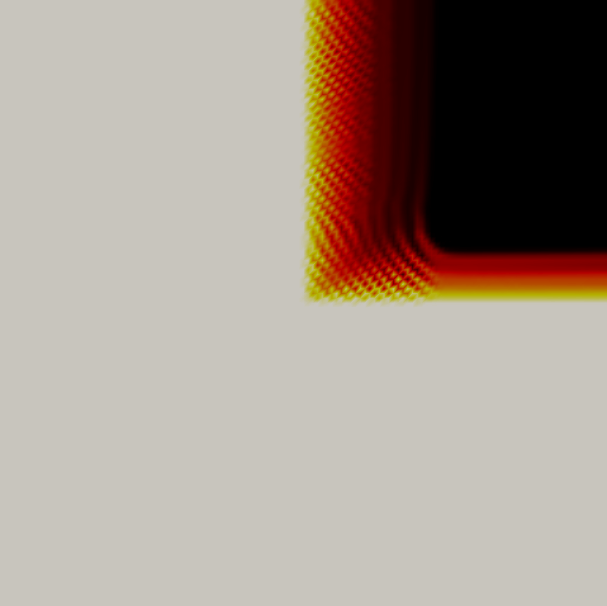
\includegraphics[width=\textwidth]
        {\contentdir/results/transport/glance_in_void/images/GalFCT_FE.png}
      \caption{Galerkin-FCT}
   \end{subfigure}
   \begin{subfigure}{0.45\textwidth}
      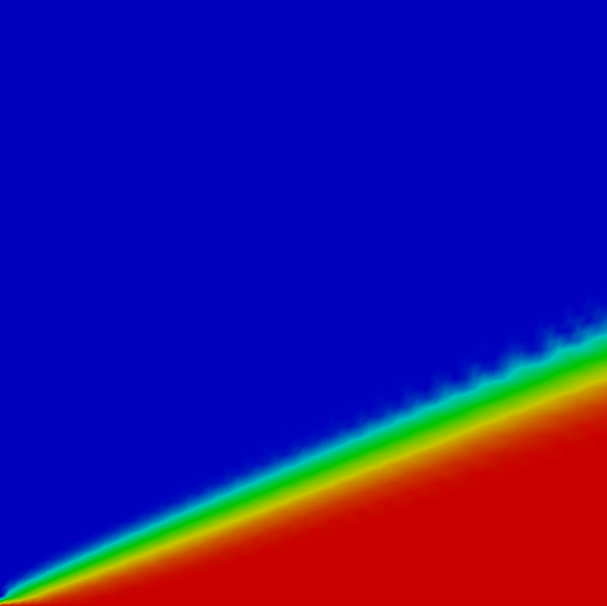
\includegraphics[width=\textwidth]
        {\contentdir/results/transport/glance_in_void/images/EVFCT_FE_cE1.png}
      \caption{EV-FCT, $\entropyresidualcoef=1.0$}
   \end{subfigure}
   \caption{Comparison of Solutions for the Glance-in-Void Test
     Problem Using Explicit Euler Time Discretization with 4096 Cells}
   \label{fig:glance_in_void_fe}
\end{figure}
%-------------------------------------------------------------------------------
\begin{figure}[ht]
   \centering
   \begin{subfigure}{0.3\textwidth}
      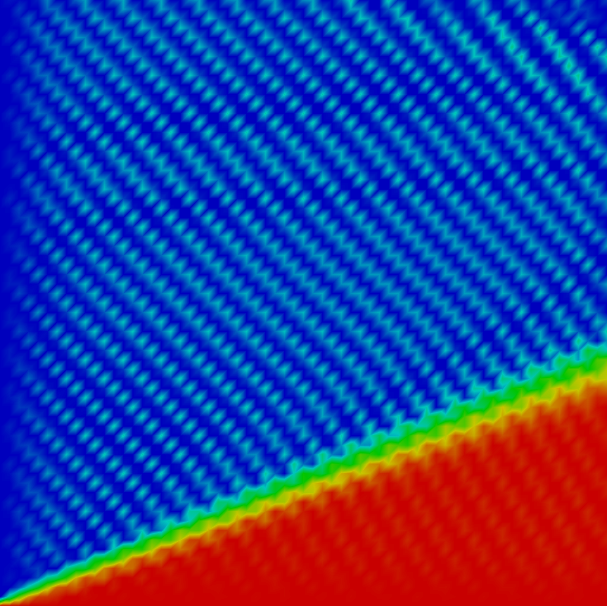
\includegraphics[width=\textwidth]
        {\contentdir/results/transport/glance_in_void/images/EV_FE_cE01.png}
      \caption{EV, $\entropyresidualcoef=0.1$}
   \end{subfigure}
   \begin{subfigure}{0.3\textwidth}
      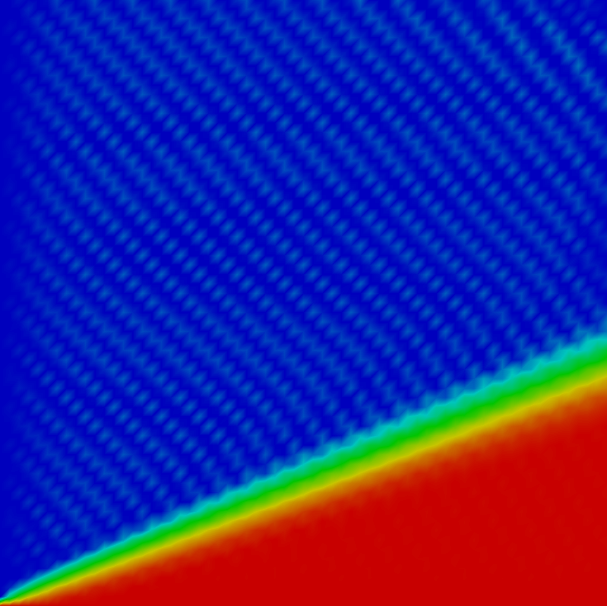
\includegraphics[width=\textwidth]
        {\contentdir/results/transport/glance_in_void/images/EV_FE_cE05.png}
      \caption{EV, $\entropyresidualcoef=0.5$}
   \end{subfigure}
   \begin{subfigure}{0.3\textwidth}
      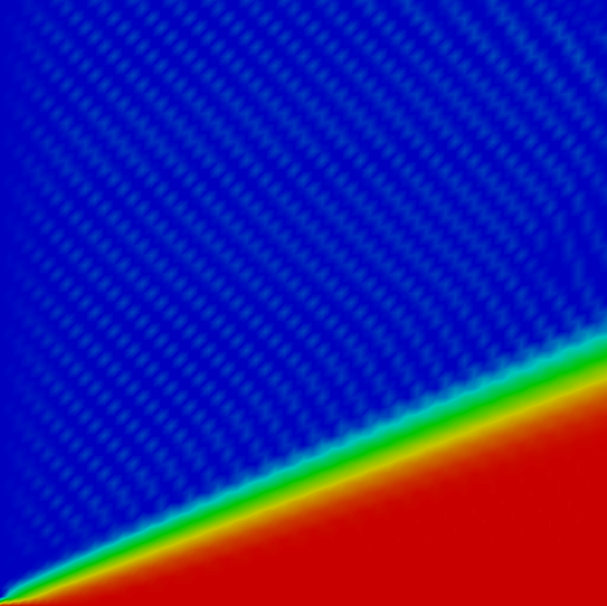
\includegraphics[width=\textwidth]
        {\contentdir/results/transport/glance_in_void/images/EV_FE_cE1.png}
      \caption{EV, $\entropyresidualcoef=1.0$}
   \end{subfigure}
   \begin{subfigure}{0.3\textwidth}
      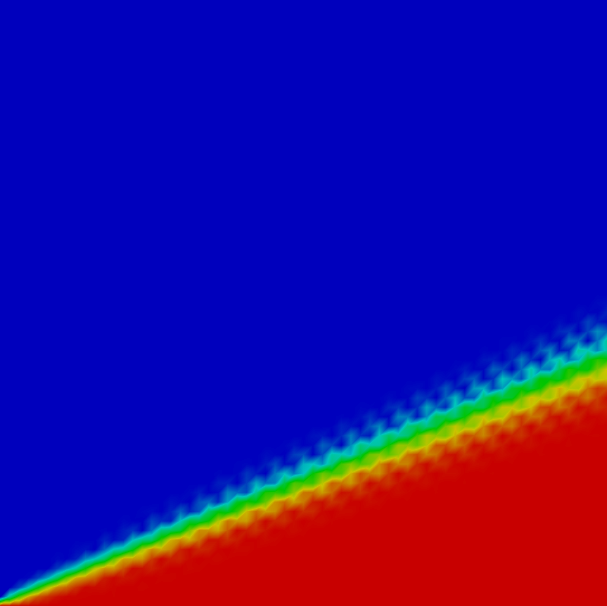
\includegraphics[width=\textwidth]
        {\contentdir/results/transport/glance_in_void/images/EVFCT_FE_cE01.png}
      \caption{EV-FCT, $\entropyresidualcoef=0.1$}
   \end{subfigure}
   \begin{subfigure}{0.3\textwidth}
      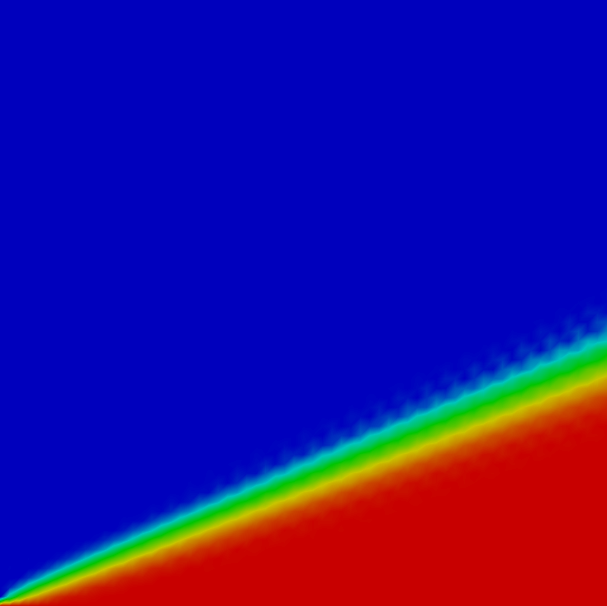
\includegraphics[width=\textwidth]
        {\contentdir/results/transport/glance_in_void/images/EVFCT_FE_cE05.png}
      \caption{EV-FCT, $\entropyresidualcoef=0.5$}
   \end{subfigure}
   \begin{subfigure}{0.3\textwidth}
      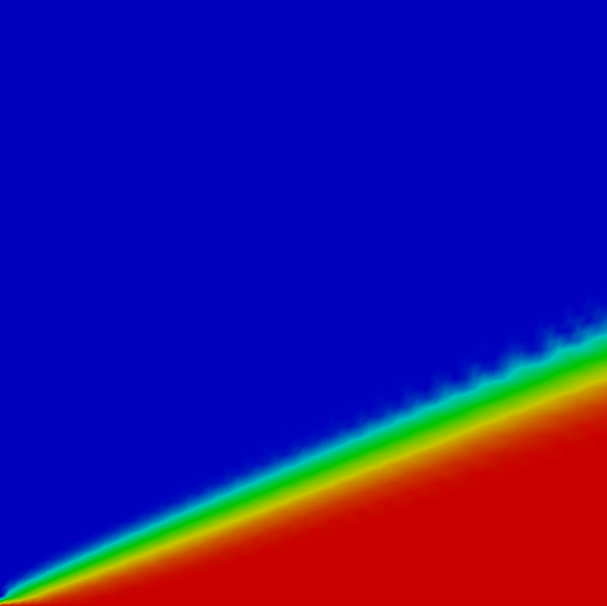
\includegraphics[width=\textwidth]
        {\contentdir/results/transport/glance_in_void/images/EVFCT_FE_cE1.png}
      \caption{EV-FCT, $\entropyresidualcoef=1.0$}
   \end{subfigure}
   \caption{Comparison of EV and EV-FCT Solutions for the Glance-in-Void Test
     Problem Using Explicit Euler Time Discretization with 4096 Cells
     and Various $\entropyresidualcoef$ Values}
   \label{fig:glance_in_void_fe_cE}
\end{figure}
%-------------------------------------------------------------------------------
\begin{figure}[ht]
   \centering
   \begin{subfigure}{0.45\textwidth}
      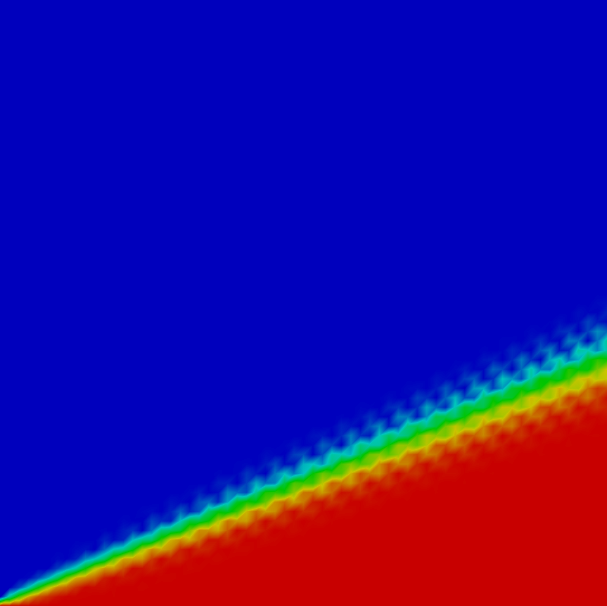
\includegraphics[width=\textwidth]
        {\contentdir/results/transport/glance_in_void/images/EVFCT_FE_cE01.png}
      \caption{EV-FCT, FE, $\entropyresidualcoef=0.1$}
   \end{subfigure}
   \begin{subfigure}{0.45\textwidth}
      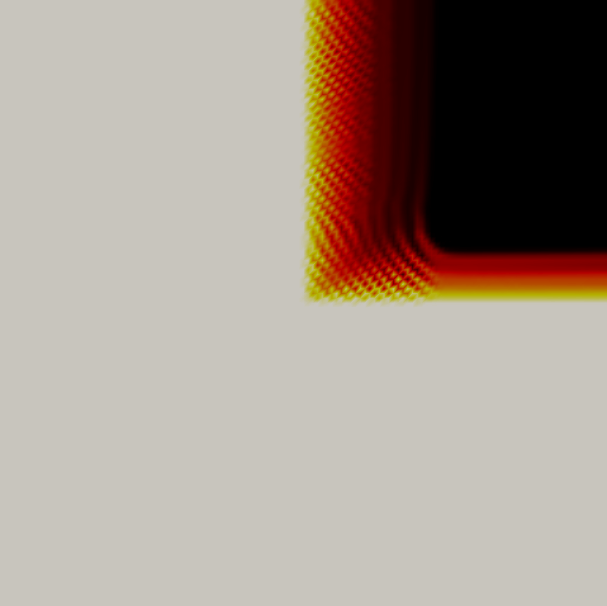
\includegraphics[width=\textwidth]
        {\contentdir/results/transport/glance_in_void/images/GalFCT_FE.png}
      \caption{Galerkin-FCT, FE}
   \end{subfigure}
   \begin{subfigure}{0.45\textwidth}
      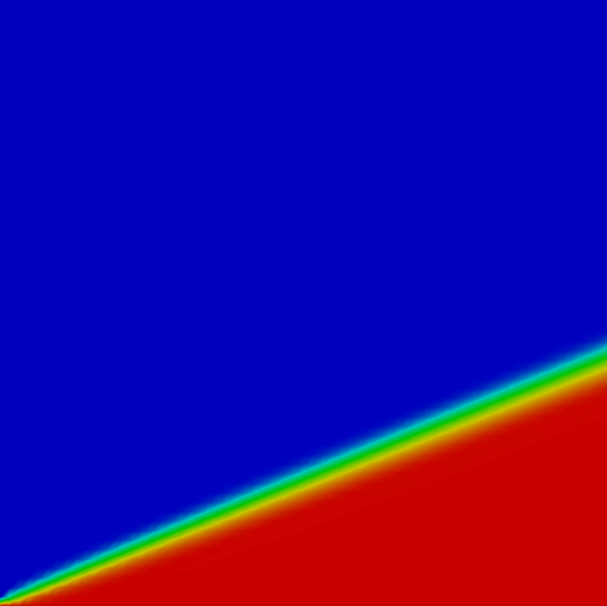
\includegraphics[width=\textwidth]
        {\contentdir/results/transport/glance_in_void/images/EVFCT_SSP3_cE01.png}
      \caption{EV-FCT, SSPRK33, $\entropyresidualcoef=0.1$}
   \end{subfigure}
   \begin{subfigure}{0.45\textwidth}
      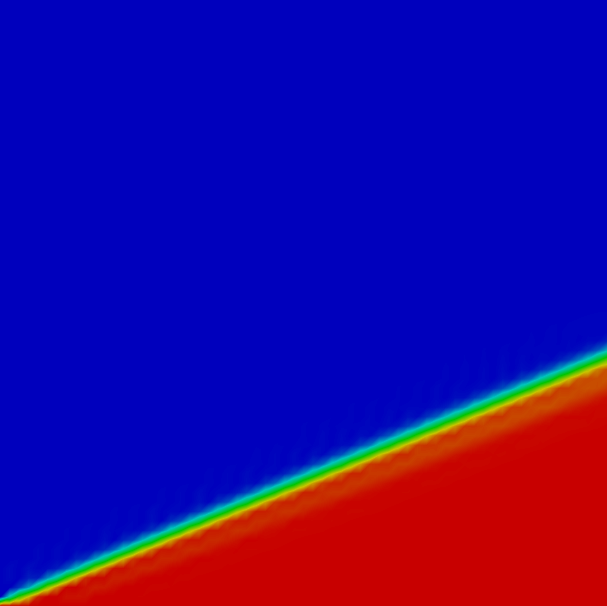
\includegraphics[width=\textwidth]
        {\contentdir/results/transport/glance_in_void/images/GalFCT_SSP3.png}
      \caption{Galerkin-FCT, SSPRK33}
   \end{subfigure}
   \caption{Comparison of Solutions for the Glance-in-Void Test
     Problem Using Explicit Euler vs. SSPRK33 with 4096 Cells}
   \label{fig:glance_in_void_fe_vs_ssprk}
\end{figure}
%-------------------------------------------------------------------------------

\clearpage

